\chapter{Implementering og Test}
\label{ch:Implementering og test af Algoritmerne}

I dette afsnit testes algoritmerne fra afsnit \ref{ch:Sorteringsalgoritmer}. Algoritmerne implementeres i python.

\section{Python}
\label{sec:Python}

Sproget Python har et højt abstraktionsniveau, og kan på mange punkter ligne vores pseudokode fra tidligere \cite[s. 68]{aogd}. Det betyder at vi på mange punkter opgiver lidt kontrol til compileren, for at gøre koden mere læsbar og tilgængelig. Det betyder også at vi aldrig helt kan vide hvilke instruktioner computeren udfører. Derudover er Python et relativt langsomt sprog, da koden kompileres samtidigt med at programmet kører. Dette gør at sproget ikke egner sig særligt godt til at skrive optimiserede algoritmer, der skal køre på meget store datasæt. Heldigvis kan vi se bort fra dette, da vi med store-O-analyse er ligeglade med den reelle udførelsestid, og i stedet er interesseret i vækstrater. Vækstraten for en algoritme er nemlig egns for en algoritme, ligegyldigt hvor langsomt hvert skridt er. På nogle punkter er det måske endda en fordel, at algoritmerne køre langsommere, da det vil gøre forskellen i udførelsestiderne større, og lettere at forholde sig til. 


\section{Implementering}
\label{sec:Implementering}

Implementering i Python er relativt simpelt. Den største forskel er at man tæller fra $1$ i pseudokode, og fra $0$ i Python (ligesom de fleste andre sprog). Det betyder for eksempel at det første element i en liste i Python er $liste[0]$, hvor det i pseudokode ville være $liste[2]$. Lykken i insertionsort der starter på $i = 2$ (se linje $\red{2}$ figur \ref{fig:Pseudokode til insertionsort}), starter  derfor i stedet på $i = 1$ i python. En anden forskel er at Python bruger dynamiske variabler \cite{what-is-python}; det er ikke nødvendigt at fortælle Python, om en variabel f.eks. er et heltal eller en liste.

\begin{figure}
	\begin{center}
		\lstinputlisting{../python/algoritmer/insertionsort.py}
	\end{center}
	\caption{Insertionsort i Python}
	\label{fig:Insertionsort i Python}
\end{figure}

\section{Test af Sorteringsalgoritmer}
\label{sec:Kode til Test af Sorteringsalgoritmer}

For at teste sorteringsalgoritmerne fra afsnit \ref{ch:Sorteringsalgoritmer}, og se hvordan deres reelle udførelsestid som funktion af $n$, relaterer til deres teoretiske væksthastighed og store-O-analyse. På figur \ref{fig:Kode til test af algoritmerne} ses koden til test af algoritmerne. Variablen $functions$ på linje $1$ indeholder en liste med de algoritmer der skal testes. I vores tilfælde indeholdt den $[insertionsort,mergesort]$. Inde in denne lykke tester vi funktionerne. Dette sikrer at algoritmerne bliver testet på samme måde. Det næste vi gør er at definere lister til opbevarting af kardinaliteten af den liste som algoritmen sorterer (l. $4$), og en til den reelle tid det tig for algoritmen at sortere listen (l. 9).  I linje $9$ sætter vi frøet for de pseudotilfældige tal \cite{python-random}, som vi senere skal bruge til at generere listerne som vi får sorteringsalgoritmerne til at sortere. Det er vigtigt af vi her sætter frøet til den samme værdi, før vi tester hver algoritme, da vi på den måde sikrer os at det er de samme pseudotilfældige lister, som algorimerne sorterer. På den måde kan vi med god vilje sammenligne algoritmernes køretider, da vi er sikre på at deres input, var det samme under testen. Efter denne \red{initialisering } begynder vi to løkker (l. 12 og 15). Den første sørger for at vi gentager den samme test flere gange. I vores tilfælde er variablen $trials$ sat til $15$, hvilket resulterer i at vi tester sorteringen af en $n$ lang liste $15$ gange. Den indre løkke tæller fra $i=0$ til $i=80$. Vi bruger herefter $i$-værdien til at generere vores $n$-værdier i linje $18$. Her bruges formlen $n=\nint{1.1^i}$. Valget at test med exponentielt stigende $n$, er af to grunde: det kan tage lang tid for en algoritme, at sortere lister med store $n$, så gør hele processen meget hurtigere, hvis man ikke tester så mange sorteringer med store $n$. Den anden og nok bedre grund, er at vi er meget interesserede i at se hvordan algoritmerne måles med hinanden, når $n$ \emph{ikke} er stort. Det ville jo være interesseret, hvis vi kunne identificere et $n_0$ som i afsnit \ref{ch:Algoritmers Udførelsestid}. Til dette skal vi bruge en punkttæthed der ved store $n$ ville være overflødig. Nu er det hele sat op, og vi kan time algoritmen på en $n$ lang liste med tilfældige tal. $n$-værdien og den tid sorteringen tog, gemmes i listerne, og eksporteres til en csv fil til brug i databehandlingen (se bilag 1 og 2).



\begin{figure}
	\begin{center}
		%\lstinputlisting[language=Python]{../python/algoritmer/mergesort.py}
		\lstinputlisting[firstline=57,lastline=85]{../python/sorting.py}
	\end{center}
	\caption{Kode til test af algoritmerne. Variablen $functions$ er en liste med de to algoritmer der testes ([insertionsort,mergesort]).}
	\label{fig:Kode til test af algoritmerne}
\end{figure}



\section{De Reelle Udførelsestider}
\label{sec:De Reelle Køretider}

Algoritmernes udførelsestider er plottet i figur \ref{fig:plot - to algoritmer}.

\subsection{Store-O er Værste Tilfælde}%
\label{sub:Store-O er Værste Tilfælde}

...grunden til at bruge algoritmens gennemsnitlige udførelsestid er...

% Plot gennemsnit for hvert n

% mergesort kører altid med store Theta(n)

\section{Optimering af Mergesort}%
\label{sub:Optimering af Mergesort}

Det er tydeligt at mergesort er langt bedre, til at sortere store lister, men ved små $n$ kan vi også se at insertionsort, ikke er langt bagefter. Faktisk er den \emph{gennemsnitlige} sortering hurtigere eller nogenlunde egens før $n = \red{15}$. Dette punkt er hvad svarer til $n_0$ fra afsnit \ref{ch:Algoritmers Udførelsestid}. At insertionsort faktisk normalt er hurtigere end mergesort hvis $n < n_0$, betyder at den mest hurtigste måde at sortere en liste afhænger af listens længde: Her listen på under $n_0$ elementer? så brug insertionsort. Er listen over $n_0$ elementer? så er mergesort gennemsnitligt hurtigere. Dette kunne lede os til at lave en ny sorteringsalgoritmerne således:

\begin{figure}[h]
	\begin{center}
		\begin{lstlisting}
		def sort(liste) {
			if liste.length <= 15 {
				return(insertionsort(liste))
			}
			return(mergesort(liste))
		}
		\end{lstlisting}
	\end{center}
	\vspace{-6mm}
	\caption{Algoritme der bruger insertionsort hvis inputlisten er kortere end $15$, og ellers mergesort.}
	\label{fig:hybridalgoritme1}
\end{figure}


Her bruger vi insertionsort hvis listens længde er under eller lig $15$, og mergesort hvis ikke. Det er en forbedrig af algoritmen. Dog er der en endnu mere snedig måde at inkorporere denne ide. Hvis vi tænker tilbage på mergesorts procedure fra afsnit \ref{ch:Sorteringsalgoritmer}, ved vi at algoritmen deler en usorterede liste op indtil der kun er lister med enkle elementer tilbage. Funktionen $merge$ sætter herefter listerne sammen igen, og sørger for at den samlede liste altid vil være sorteret, da den altid for sorterede lister som input. Vi ved dog nu at denne process, ikke er effektiv ved $n$-værdier under \red{15 }. Det er derfor en smart ide at bruge insertionsort til at sortere listerne når mergesort har opdelt listen i tilstrækkeligt små bidder. Koden for denne hybridalgoritme kan ses på figur \ref{fig:hybridalgoritme2}. I stedet for at opdele listen helt til der kun er et enkelt element i hver delliste, stopper denne algoritme opdelingen så snart insertionsort kan sortere listen hurtigere.

\subsection{Sammenligning af Optimerede Algoritmer}%
\label{sub:Sammenligning af Optimerede Algoritmer}



\begin{figure}
	\begin{center}
		\lstinputlisting[lastline=23]{../python/algoritmer/mergesort_optimized.py}
	\end{center}
	\caption{Mergesort hvor lister mindre end \red{15 } sorteres effektivt af insertionsort}
	\label{fig:hybridalgoritme2}
\end{figure}



\begin{figure} \centering
	\begin{subfigure}[b]{0.45\textwidth}
		\centering
		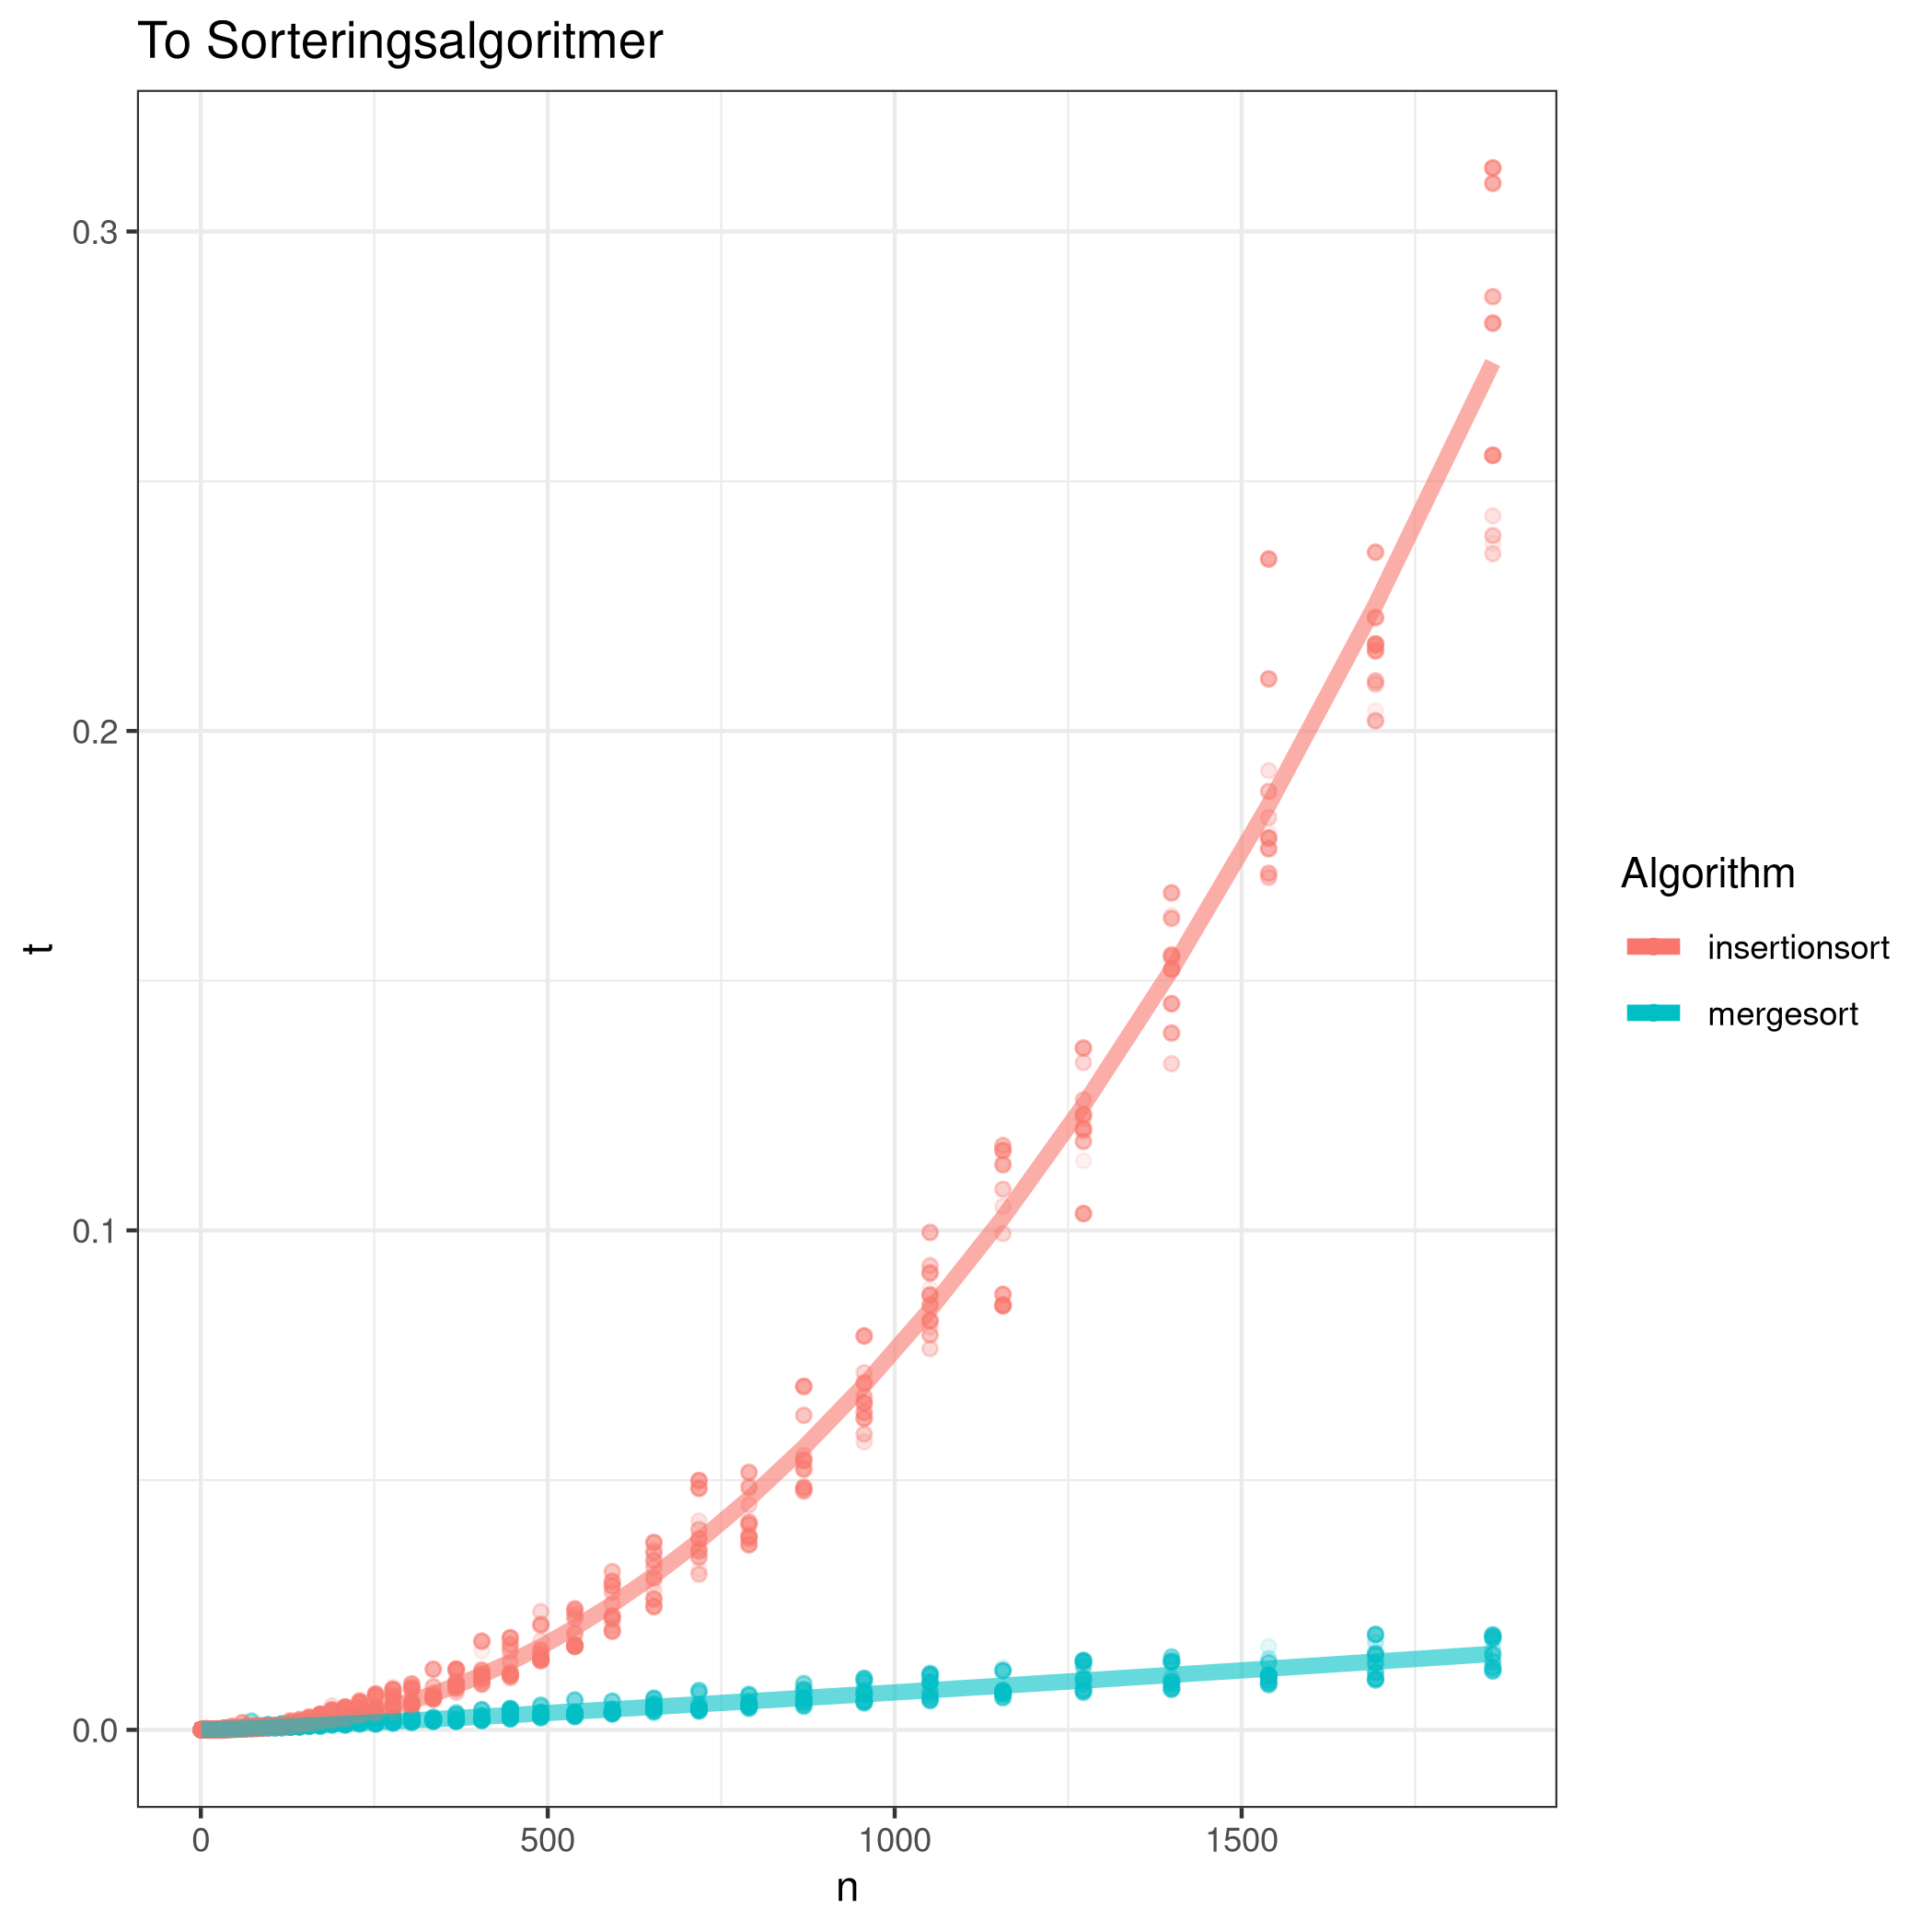
\includegraphics[width=\textwidth]{../img/toAlgoritmer.png}
		\caption{$y=\input{../img/r2-insertion.txt}$}
		\label{fig:regressioner}
	\end{subfigure}
	\hfill
	\begin{subfigure}[b]{0.45\textwidth}
		\centering
		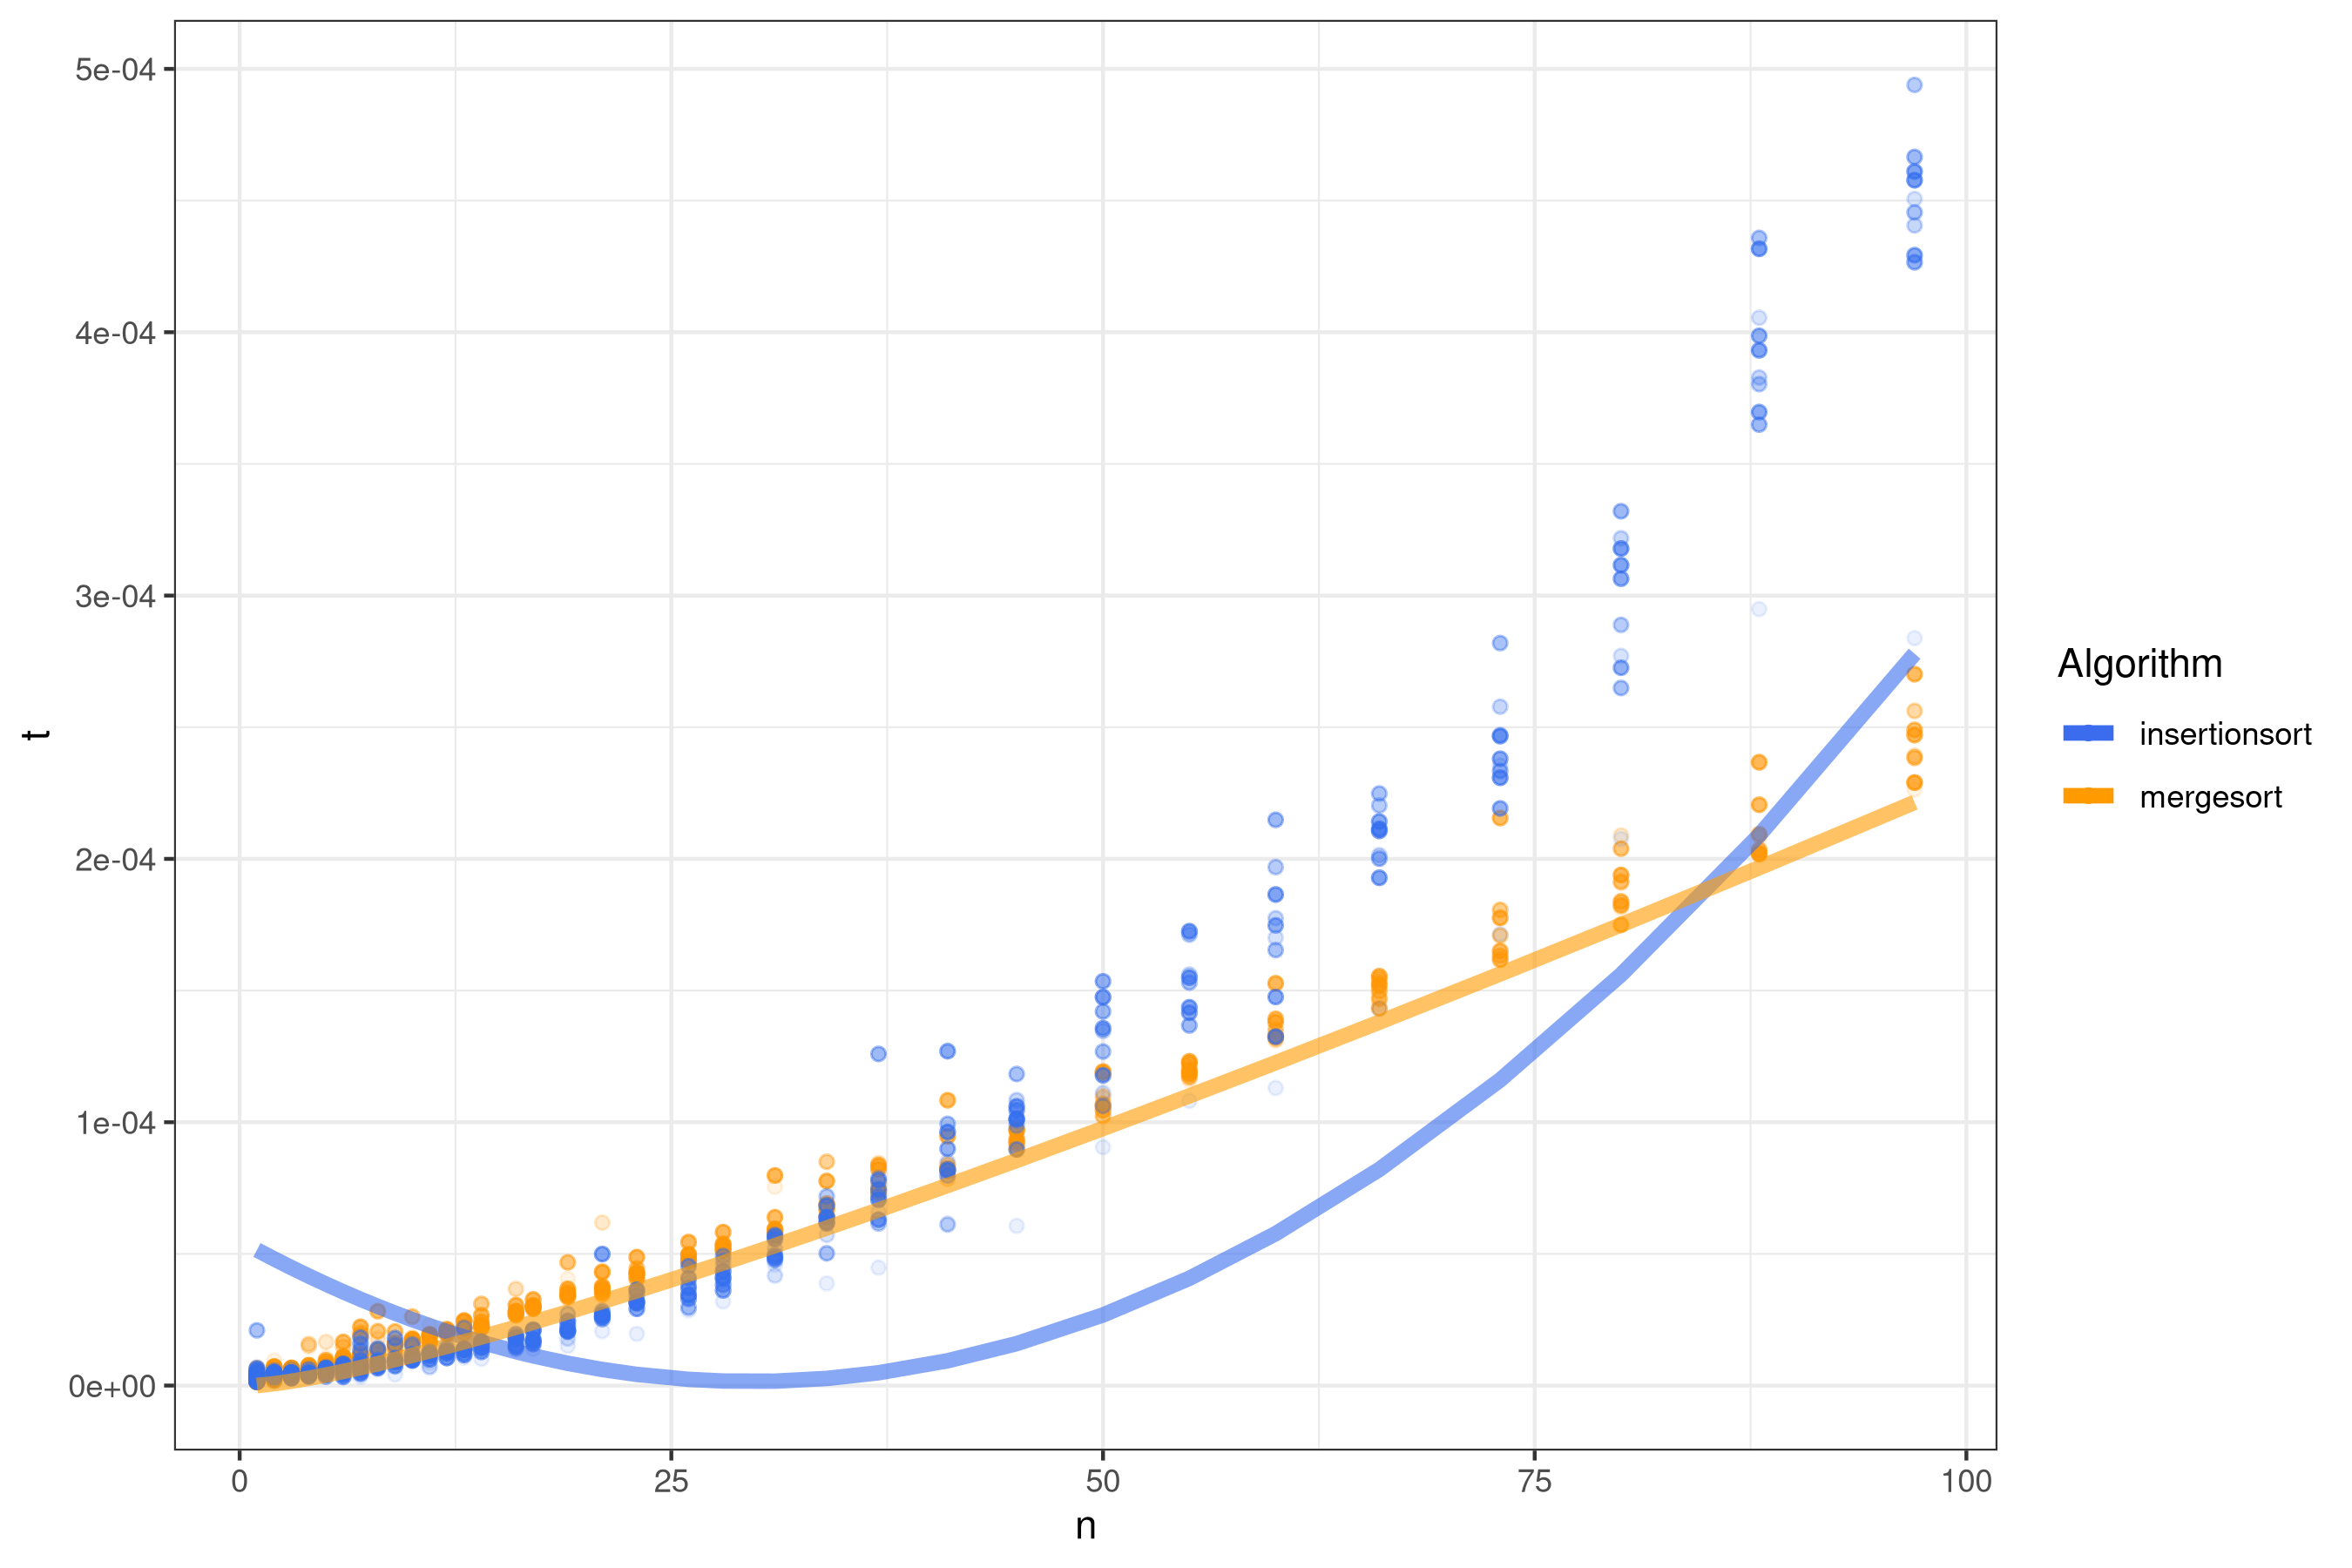
\includegraphics[width=\textwidth]{../img/toAlgoritmerZoomed}
		\caption{$y=3sinx$}
		\label{fig:residualplot}
	\end{subfigure}
	\caption{Sammenligning af insertionsort og mergesort}
	\label{fig:plot - to algoritmer}
\end{figure}
